\documentclass[a4paper,11pt]{article}
%@@@@@@@@@@@@@@@@@@@@@@@@@@@@@@@@@@@@@@@@@@@@@@@@@@@@@@@@@@@
%@@@@@@@@@@@@@@@@      PACOTES BÁSICOS		     @@@@@@@@@@
%@@@@@@@@@@@@@@@@@@@@@@@@@@@@@@@@@@@@@@@@@@@@@@@@@@@@@@@@@@@

\usepackage[T1]{fontenc}
\usepackage[utf8]{inputenc}
\usepackage{lmodern} 
\usepackage[portuguese]{babel}
\usepackage{amsmath}
\usepackage{array}
\usepackage{graphicx}				%para imagens
\usepackage{epstopdf} 				%resolve problemas eps-pdf
\usepackage{pict2e}				%%writting to images
%@@@@@@@@@@@@@@@@@@@@@@@@@@@@@@@@@@@@@@@@@@@@@@@@@@@@@@@@@@@
%@@@@@@@@@@@@@@@@     PACOTES NÃO TAOBÁSICOS		 @@@@@@@@@@
%@@@@@@@@@@@@@@@@@@@@@@@@@@@@@@@@@@@@@@@@@@@@@@@@@@@@@@@@@@@
\usepackage{fancyhdr}				% para o cabeçalho bonito
\usepackage{caption}					%para legendas
\usepackage{subcaption}				% e sublegendas
\usepackage{placeins} 				%controlar o lugar dos floats
\pagestyle{fancy} 					% número de pag e cabeçalho
\usepackage{txfonts} 				%fontes bonitas? acho que para o título
\usepackage[usenames]{color} 		% algo com gunplot e eps
\usepackage{ifthen}
\usepackage{xparse}
\graphicspath{{./../images/}{./../data/}{./graph/}}	% procura imagens nessa pasta
\usepackage{float} %%para definir ambiente gráfico
\newfloat{Gráfico}{hbtp}{lop}[section]
%\usepackage{undertilde}	%%para notação de vetor do yuri
\usepackage[import]{xy} % para escrever em imagens
\xyoption{import}

\usepackage{listings}
\lstset{frame=single,}
%@@@@@@@@@@@@@@@@@@@@@@@@@@@@@@@@@@@@@@@@@@@@@@@@@@@@@@@@@@@
%@@@@@@@@@@@@@@@@      Cabeçalho de cada página      @@@@@@@
%@@@@@@@@@@@@@@@@@@@@@@@@@@@@@@@@@@@@@@@@@@@@@@@@@@@@@@@@@@@
\setlength{\headheight}{25pt}%compila sem erro
	\fancyhead{}
	\fancyfoot{}
	\fancyhead[R]{Sistemas de Medição}%direito superior
	\fancyhead[L]{
\includegraphics[height=0.25in]{./../images/logo_unb.pdf}}%esquerda superior
	\fancyfoot[C]{\thepage}%baixo centro
%E: Even page, O: Odd page, L: Left field, C: Center field, R: Right field, H: Header, F: Footer
% em documentos com dois lados use LO, RO. como esse documento não tem lados essa opção é inútil


%@@@@@@@@@@@@@@@@@@@@@@@@@@@@@@@@@@@@@@@@@@@@@@@@@@@@@@@@@@@
%@@@@@@@@@@@@@@@@      NOVOS COMANDOS		      @@@@@@@@@
%@@@@@@@@@@@@@@@@@@@@@@@@@@@@@@@@@@@@@@@@@@@@@@@@@@@@@@@@@@@
\newcommand\undermat[2]
	{
	  \makebox[0pt][l]
	  	{$\smash{\underbrace{\phantom{%
    \begin{matrix}#2\end{matrix}}}_{\text{$#1$}}}$
    		}#2
    	}
    	
\newcommand{\HRule}
	{
	\rule{\linewidth}{0.5mm}
	}
	
\newcommand{\EmptyPage}
	{
	\thispagestyle{empty}
	\mbox{ }
	\newpage	
	} 
	
\newcommand{\MakeMyTitlePage}[4]
%%Argumentos: 
%1º Nome da Matéria
%2º subtítulo ex: experimento IV
%3º título
%4º autores
% exemplo de autores:
%	\begin{center} \large
%		\begin{tabular}{llr} \
%		& & \\[0.05cm]		
%		Professora & Nadia Maria de Liz Koche & \\
%		
%		Alunos:& & \\
%		& Juarez A.S.F 					& 11/0032829\\
%		& Sérgio Fernandes da Silva Reis & 11/0140257\\
%		& Jedhai Pimentel				& 09/0007883\\	[0.05cm]	
%		\end{tabular}
%	\end{center}
{
\begin{titlepage}
\begin{center}

% Upper part of the page. The '~' is needed because \\
% only works if a paragraph has started.

\includegraphics[width=\textwidth]{./../images/logo_unb.pdf}~\\[1cm]

\Huge #1\\[0.5cm]

\huge #2

% Title
\HRule \\[0.4cm]
{ \huge \bfseries  #3}\\[0.4cm]

\HRule \\[0.5cm]

{\large \today}


\vfill %%o que vier depois vai ao fim da páginda


%Autor e Professor
\begin{center} \large
#4
\end{center}

\end{center}
\end{titlepage}

\EmptyPage
\tableofcontents
\newpage

}
	
%@@@@@@@@@@@@@@@@@@@@@@@@@@@@@@@@@@@@@@@@@@@@@@@@@@@@@@@@@@@
%@@@@@@@@@@@@@@@@      NOVOS AMBIENTES		      @@@@@@@@@
%@@@@@@@@@@@@@@@@@@@@@@@@@@@@@@@@@@@@@@@@@@@@@@@@@@@@@@@@@@@
\newcounter{graph-c}
\setcounter{graph-c}{0}


%\NewDocumentEnvironment{Graph}{m}
 % {%antes
  %\addtocounter{graph-c}{1}
  %\begin{figure}
  %}
 %{
 %depois
%	\end{figure} 
%	\caption*{Grafico \arabic{graph-c} - #1}
 %}

















%inclui todosos pacotes utilizados


\begin{document}

\begin{titlepage}
\begin{center}

% Upper part of the page. The '~' is needed because \\
% only works if a paragraph has started.

\includegraphics[width=\textwidth]{logo_unb.pdf}~\\[1cm]

\Huge Física Experimental 4\\[0.5cm]

\huge Experimento III

% Title
\HRule \\[0.4cm]
{ \huge \bfseries  Decaimento da Intensidade Luminosa e Coeficientes de Absorção e Reflexão}\\[0.4cm]

\HRule \\[0.5cm]

{\large \today}


\vfill %%o que vier depois vai ao fim da páginda


% Author and supervisor

	\begin{center} \large
		\begin{tabular}{llr} \
		& & \\[0.05cm]		
		Professora & Nadia Maria de Liz Koche & \\
		
		Alunos:& & \\
		& Juarez A.S.F 					& 11/0032829\\
		& Sérgio Fernandes da Silva Reis & 11/0140257\\
		& Jedhai Pimentel				& 09/0007883\\	[0.05cm]	
		\end{tabular}

	
	\end{center}


\end{center}
\end{titlepage}
\EmptyPage

\section{Resumo}
\paragraph{} Apresenta-se o uso de diferenças finitas para resolver a equação de Laplace na forma homogênea e não homogênea(eq. de Poisson) nas condições de Neuman e Dirichlet.

\section{Introdução}
\paragraph{}Presente em muitas aplicações matemáticas a equação de Laplace é uma equação diferencial parcial da forma:
\begin{equation}
	\nabla ^2 \phi = \del{x}{2} \phi + \del{y}{2} \phi = 0
\end{equation}
\paragraph{}A equação deve ser válida no interior de um domínio $\Omega$ e sobre as bordas do domínio $\borda$ devem valer as chamadas condições de contorno. Estas últimas assumem em geral três principais formas:
\begin{itemize}
	\item condição de \textbf{Dirichlet}: quando especifica-se a função sobre a fronteira. Ex.: $\phi (x,y) = f(x,y)$ sobre $\borda$.
	\item condição de \textbf{Neuman}: quando especifica-se a derivada normal à fronteira da função. Ex.: $\frac{\partial}{\partial n} \phi$ sobre $\borda$  
	\item condição de \textbf{Robin}: especifica-se uma combinação linear das função e sua derivada normal sobre $\borda$. Ex.: $\phi + \frac{\partial}{\partial n} \phi =  0$ sobre $\borda$. 
\end{itemize}

\paragraph{} Apenas para exemplificar esses três tipos de condição de contorno considere o problema de calor em uma barra finita. Considerado o processo unidimensional para simplificação a equação que o governa é: 
\begin{equation}
	\del{t}{1} u(x,t) = k \del{x}{2} u(x,t)
\end{equation}
\paragraph{}Onde k é a constante de transmissividade térmica. Um exemplo de condição de \textbf{Dirichlet} associada seria mergulhar a extremidade $x = 0$ da barra em gelo e a outra $x = L$ em vapor d'água. Dessa forma estamos especificando a função em suas fronteiras. Junto com uma condição inicial $u(x, 0)$ o problema está bem posto e pode ser modelado como:
\begin{equation}
\left\{ 
	\begin{array}{l}
	\del{t}{1} u(x,t) = k \del{x}{2} u(x,t) \\
	u(0, t) = 0 \\
	 u(L, t) = 100 \\
	u(x, 0) = f(x)
	\end{array}
\right.
\end{equation}
\paragraph{} A condição de \textbf{Neuman} para esse mesmo problema seria, por exemplo, adicionar uma bomba de calor como um maçarico em uma das extremidades. Dessa forma essa extremidade teria sua derivada normal, no caso a derivada em relação a x, especificada. 

\paragraph{}A equação do calor foi citada apenas a título de exemplificação mas podemos comparar os dois problema para obtermos observações importantes. A equação de Laplace não envolve derivada temporal e portanto não precisa de uma condição inicial como a equação do calor. A solução depende exclusivamente da equação, das condições de contorno e da geometria do problema.

\paragraph{}Na aplicação que temos em mente a equação de Laplace não-homogênea(\textbf{eq. de Poisson}) aparece no algoritmo de solução numérica para a equação de Navier-Stokes. Mais especificamente, para o cálculo da pressão do sistema. O problema será resolvido em um domínio retangular sob condições de contorno de \textbf{Neuman} em todos os lados. Nesse caso, com 4 condições de \textbf{Neuman}, o problema não tem solução única mas em nossa aplicação isso não será um problema, visto que a pressão aparece na equação com sua derivada espacial.

\section{Diferenças Finitas}

\paragraph{}Consiste em uma discretização de um operador diferencial. A construção segue da fórmula de Taylor e permite avaliar as derivadas de uma função como uma combinação linear dos valores da função em pontos próximos e no próprio ponto considerado. O método pode ser entendido como uma aproximação numérica para as derivadas. Como se trata de uma aproximação podemos avaliar o erro da aproximação em função de quão próximos estão os pontos considerados. As diversas fórmulas utilizadas no método possuem cada uma um erro associado $O(h)$ que medem o quão rápido nossa aproximação se aproxima do valor exato a medida que nos aproximamos de h = 0. Um algoritmo que tenha $O(h^2)$ é dito de segunda ordem. Consideramos aqui as aproximações por diferenças finitas de segunda ordem para as derivadas primeira e segundas.

\paragraph{}Seja $u(x,y):\Re^2 \longrightarrow \Re$. 


\section{Resultados}
\paragraph{}Seguem alguns resultados obtidos.

\begin{Gráfico}
	% GNUPLOT: LaTeX picture with Postscript
\begingroup
  \fontfamily{phv}%
  \selectfont
\definecolor{t}{rgb}{0.5,0.5,0.5}
  \makeatletter
  \providecommand\color[2][]{%
    \GenericError{(gnuplot) \space\space\space\@spaces}{%
      Package color not loaded in conjunction with
      terminal option `colourtext'%
    }{See the gnuplot documentation for explanation.%
    }{Either use 'blacktext' in gnuplot or load the package
      color.sty in LaTeX.}%
    \renewcommand\color[2][]{}%
  }%
  \providecommand\includegraphics[2][]{%
    \GenericError{(gnuplot) \space\space\space\@spaces}{%
      Package graphicx or graphics not loaded%
    }{See the gnuplot documentation for explanation.%
    }{The gnuplot epslatex terminal needs graphicx.sty or graphics.sty.}%
    \renewcommand\includegraphics[2][]{}%
  }%
  \providecommand\rotatebox[2]{#2}%
  \@ifundefined{ifGPcolor}{%
    \newif\ifGPcolor
    \GPcolortrue
  }{}%
  \@ifundefined{ifGPblacktext}{%
    \newif\ifGPblacktext
    \GPblacktextfalse
  }{}%
  % define a \g@addto@macro without @ in the name:
  \let\gplgaddtomacro\g@addto@macro
  % define empty templates for all commands taking text:
  \gdef\gplbacktext{}%
  \gdef\gplfronttext{}%
  \makeatother
  \ifGPblacktext
    % no textcolor at all
    \def\colorrgb#1{}%
    \def\colorgray#1{}%
  \else
    % gray or color?
    \ifGPcolor
      \def\colorrgb#1{\color[rgb]{#1}}%
      \def\colorgray#1{\color[gray]{#1}}%
      \expandafter\def\csname LTw\endcsname{\color{white}}%
      \expandafter\def\csname LTb\endcsname{\color{black}}%
      \expandafter\def\csname LTa\endcsname{\color{black}}%
      \expandafter\def\csname LT0\endcsname{\color[rgb]{1,0,0}}%
      \expandafter\def\csname LT1\endcsname{\color[rgb]{0,1,0}}%
      \expandafter\def\csname LT2\endcsname{\color[rgb]{0,0,1}}%
      \expandafter\def\csname LT3\endcsname{\color[rgb]{1,0,1}}%
      \expandafter\def\csname LT4\endcsname{\color[rgb]{0,1,1}}%
      \expandafter\def\csname LT5\endcsname{\color[rgb]{1,1,0}}%
      \expandafter\def\csname LT6\endcsname{\color[rgb]{0,0,0}}%
      \expandafter\def\csname LT7\endcsname{\color[rgb]{1,0.3,0}}%
      \expandafter\def\csname LT8\endcsname{\color[rgb]{0.5,0.5,0.5}}%
    \else
      % gray
      \def\colorrgb#1{\color{black}}%
      \def\colorgray#1{\color[gray]{#1}}%
      \expandafter\def\csname LTw\endcsname{\color{white}}%
      \expandafter\def\csname LTb\endcsname{\color{black}}%
      \expandafter\def\csname LTa\endcsname{\color{black}}%
      \expandafter\def\csname LT0\endcsname{\color{black}}%
      \expandafter\def\csname LT1\endcsname{\color{black}}%
      \expandafter\def\csname LT2\endcsname{\color{black}}%
      \expandafter\def\csname LT3\endcsname{\color{black}}%
      \expandafter\def\csname LT4\endcsname{\color{black}}%
      \expandafter\def\csname LT5\endcsname{\color{black}}%
      \expandafter\def\csname LT6\endcsname{\color{black}}%
      \expandafter\def\csname LT7\endcsname{\color{black}}%
      \expandafter\def\csname LT8\endcsname{\color{black}}%
    \fi
  \fi
  \setlength{\unitlength}{0.0500bp}%
  \begin{picture}(7936.00,5668.00)%
    \gplgaddtomacro\gplbacktext{%
      \csname LTb\endcsname%
      \put(1005,1328){\makebox(0,0){\strut{} 0}}%
      \put(1370,1260){\makebox(0,0){\strut{} 0.1}}%
      \put(1736,1192){\makebox(0,0){\strut{} 0.2}}%
      \put(2101,1124){\makebox(0,0){\strut{} 0.3}}%
      \put(2466,1056){\makebox(0,0){\strut{} 0.4}}%
      \put(2831,988){\makebox(0,0){\strut{} 0.5}}%
      \put(3196,920){\makebox(0,0){\strut{} 0.6}}%
      \put(3561,852){\makebox(0,0){\strut{} 0.7}}%
      \put(3926,784){\makebox(0,0){\strut{} 0.8}}%
      \put(4290,716){\makebox(0,0){\strut{} 0.9}}%
      \put(4655,648){\makebox(0,0){\strut{} 1}}%
      \put(4833,696){\makebox(0,0){\strut{} 0}}%
      \put(5043,814){\makebox(0,0){\strut{} 0.1}}%
      \put(5254,932){\makebox(0,0){\strut{} 0.2}}%
      \put(5465,1050){\makebox(0,0){\strut{} 0.3}}%
      \put(5676,1168){\makebox(0,0){\strut{} 0.4}}%
      \put(5887,1286){\makebox(0,0){\strut{} 0.5}}%
      \put(6097,1404){\makebox(0,0){\strut{} 0.6}}%
      \put(6308,1522){\makebox(0,0){\strut{} 0.7}}%
      \put(6519,1640){\makebox(0,0){\strut{} 0.8}}%
      \put(6730,1758){\makebox(0,0){\strut{} 0.9}}%
      \put(6941,1876){\makebox(0,0){\strut{} 1}}%
      \put(963,2192){\makebox(0,0)[r]{\strut{}-60}}%
      \put(963,2417){\makebox(0,0)[r]{\strut{}-50}}%
      \put(963,2641){\makebox(0,0)[r]{\strut{}-40}}%
      \put(963,2865){\makebox(0,0)[r]{\strut{}-30}}%
      \put(963,3090){\makebox(0,0)[r]{\strut{}-20}}%
      \put(963,3314){\makebox(0,0)[r]{\strut{}-10}}%
      \put(963,3539){\makebox(0,0)[r]{\strut{} 0}}%
      \put(963,3763){\makebox(0,0)[r]{\strut{} 10}}%
      \put(333,2977){\makebox(0,0){\strut{}f(x,y)}}%
      \put(3968,5325){\makebox(0,0){\strut{}Solução numérica para equação de Laplace}}%
    }%
    \gplgaddtomacro\gplfronttext{%
      \csname LTb\endcsname%
      \put(6136,4884){\makebox(0,0)[r]{\strut{}n = 200}}%
      \csname LTb\endcsname%
      \put(2388,771){\makebox(0,0){\strut{}x}}%
      \put(6706,1145){\makebox(0,0){\strut{}y}}%
      \put(333,2977){\makebox(0,0){\strut{}f(x,y)}}%
      \put(7356,2433){\makebox(0,0)[l]{\strut{}-60}}%
      \put(7356,2683){\makebox(0,0)[l]{\strut{}-50}}%
      \put(7356,2934){\makebox(0,0)[l]{\strut{}-40}}%
      \put(7356,3184){\makebox(0,0)[l]{\strut{}-30}}%
      \put(7356,3435){\makebox(0,0)[l]{\strut{}-20}}%
      \put(7356,3685){\makebox(0,0)[l]{\strut{}-10}}%
      \put(7356,3936){\makebox(0,0)[l]{\strut{} 0}}%
      \put(7356,4187){\makebox(0,0)[l]{\strut{} 10}}%
    }%
    \gplbacktext
    \put(0,0){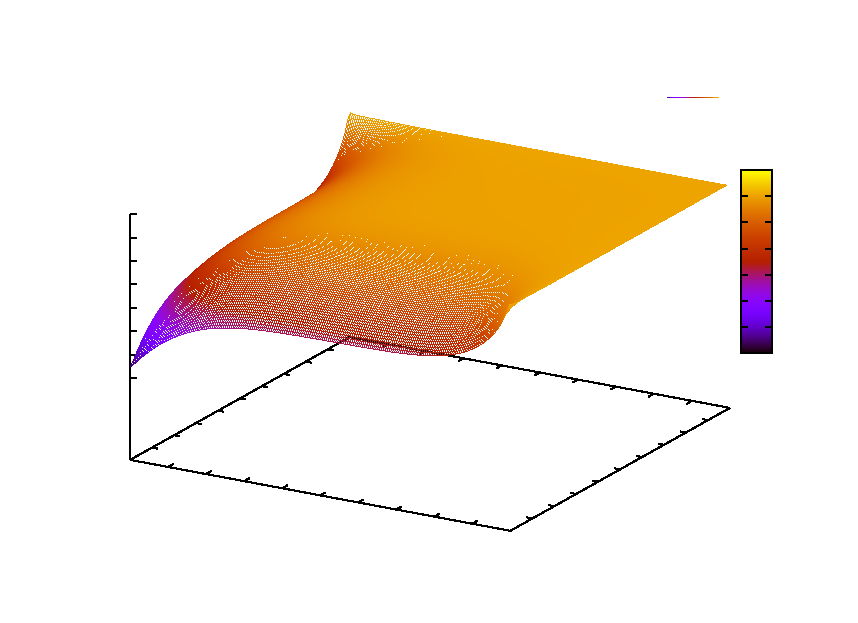
\includegraphics{./graph-01}}%
    \gplfronttext
  \end{picture}%
\endgroup

\end{Gráfico}

\begin{Gráfico}
	% GNUPLOT: LaTeX picture with Postscript
\begingroup
  \fontfamily{phv}%
  \selectfont
\definecolor{t}{rgb}{0.5,0.5,0.5}
  \makeatletter
  \providecommand\color[2][]{%
    \GenericError{(gnuplot) \space\space\space\@spaces}{%
      Package color not loaded in conjunction with
      terminal option `colourtext'%
    }{See the gnuplot documentation for explanation.%
    }{Either use 'blacktext' in gnuplot or load the package
      color.sty in LaTeX.}%
    \renewcommand\color[2][]{}%
  }%
  \providecommand\includegraphics[2][]{%
    \GenericError{(gnuplot) \space\space\space\@spaces}{%
      Package graphicx or graphics not loaded%
    }{See the gnuplot documentation for explanation.%
    }{The gnuplot epslatex terminal needs graphicx.sty or graphics.sty.}%
    \renewcommand\includegraphics[2][]{}%
  }%
  \providecommand\rotatebox[2]{#2}%
  \@ifundefined{ifGPcolor}{%
    \newif\ifGPcolor
    \GPcolortrue
  }{}%
  \@ifundefined{ifGPblacktext}{%
    \newif\ifGPblacktext
    \GPblacktextfalse
  }{}%
  % define a \g@addto@macro without @ in the name:
  \let\gplgaddtomacro\g@addto@macro
  % define empty templates for all commands taking text:
  \gdef\gplbacktext{}%
  \gdef\gplfronttext{}%
  \makeatother
  \ifGPblacktext
    % no textcolor at all
    \def\colorrgb#1{}%
    \def\colorgray#1{}%
  \else
    % gray or color?
    \ifGPcolor
      \def\colorrgb#1{\color[rgb]{#1}}%
      \def\colorgray#1{\color[gray]{#1}}%
      \expandafter\def\csname LTw\endcsname{\color{white}}%
      \expandafter\def\csname LTb\endcsname{\color{black}}%
      \expandafter\def\csname LTa\endcsname{\color{black}}%
      \expandafter\def\csname LT0\endcsname{\color[rgb]{1,0,0}}%
      \expandafter\def\csname LT1\endcsname{\color[rgb]{0,1,0}}%
      \expandafter\def\csname LT2\endcsname{\color[rgb]{0,0,1}}%
      \expandafter\def\csname LT3\endcsname{\color[rgb]{1,0,1}}%
      \expandafter\def\csname LT4\endcsname{\color[rgb]{0,1,1}}%
      \expandafter\def\csname LT5\endcsname{\color[rgb]{1,1,0}}%
      \expandafter\def\csname LT6\endcsname{\color[rgb]{0,0,0}}%
      \expandafter\def\csname LT7\endcsname{\color[rgb]{1,0.3,0}}%
      \expandafter\def\csname LT8\endcsname{\color[rgb]{0.5,0.5,0.5}}%
    \else
      % gray
      \def\colorrgb#1{\color{black}}%
      \def\colorgray#1{\color[gray]{#1}}%
      \expandafter\def\csname LTw\endcsname{\color{white}}%
      \expandafter\def\csname LTb\endcsname{\color{black}}%
      \expandafter\def\csname LTa\endcsname{\color{black}}%
      \expandafter\def\csname LT0\endcsname{\color{black}}%
      \expandafter\def\csname LT1\endcsname{\color{black}}%
      \expandafter\def\csname LT2\endcsname{\color{black}}%
      \expandafter\def\csname LT3\endcsname{\color{black}}%
      \expandafter\def\csname LT4\endcsname{\color{black}}%
      \expandafter\def\csname LT5\endcsname{\color{black}}%
      \expandafter\def\csname LT6\endcsname{\color{black}}%
      \expandafter\def\csname LT7\endcsname{\color{black}}%
      \expandafter\def\csname LT8\endcsname{\color{black}}%
    \fi
  \fi
  \setlength{\unitlength}{0.0500bp}%
  \begin{picture}(7936.00,5668.00)%
    \gplgaddtomacro\gplbacktext{%
      \csname LTb\endcsname%
      \put(882,576){\makebox(0,0)[r]{\strut{} 0}}%
      \put(882,1335){\makebox(0,0)[r]{\strut{} 1000}}%
      \put(882,2093){\makebox(0,0)[r]{\strut{} 2000}}%
      \put(882,2852){\makebox(0,0)[r]{\strut{} 3000}}%
      \put(882,3610){\makebox(0,0)[r]{\strut{} 4000}}%
      \put(882,4369){\makebox(0,0)[r]{\strut{} 5000}}%
      \put(882,5127){\makebox(0,0)[r]{\strut{} 6000}}%
      \put(990,396){\makebox(0,0){\strut{} 0.5}}%
      \put(1726,396){\makebox(0,0){\strut{} 1}}%
      \put(2461,396){\makebox(0,0){\strut{} 1.5}}%
      \put(3197,396){\makebox(0,0){\strut{} 2}}%
      \put(3933,396){\makebox(0,0){\strut{} 2.5}}%
      \put(4668,396){\makebox(0,0){\strut{} 3}}%
      \put(5404,396){\makebox(0,0){\strut{} 3.5}}%
      \put(6140,396){\makebox(0,0){\strut{} 4}}%
      \put(6875,396){\makebox(0,0){\strut{} 4.5}}%
      \put(7611,396){\makebox(0,0){\strut{} 5}}%
      \put(144,2851){\makebox(0,0){\strut{}n}}%
      \put(4300,126){\makebox(0,0){\strut{}w}}%
      \put(4300,5397){\makebox(0,0){\strut{}Número de iterações para $\epsilon =0.1$}}%
    }%
    \gplgaddtomacro\gplfronttext{%
      \csname LTb\endcsname%
      \put(6792,4974){\makebox(0,0)[r]{\strut{}n = 100}}%
    }%
    \gplbacktext
    \put(0,0){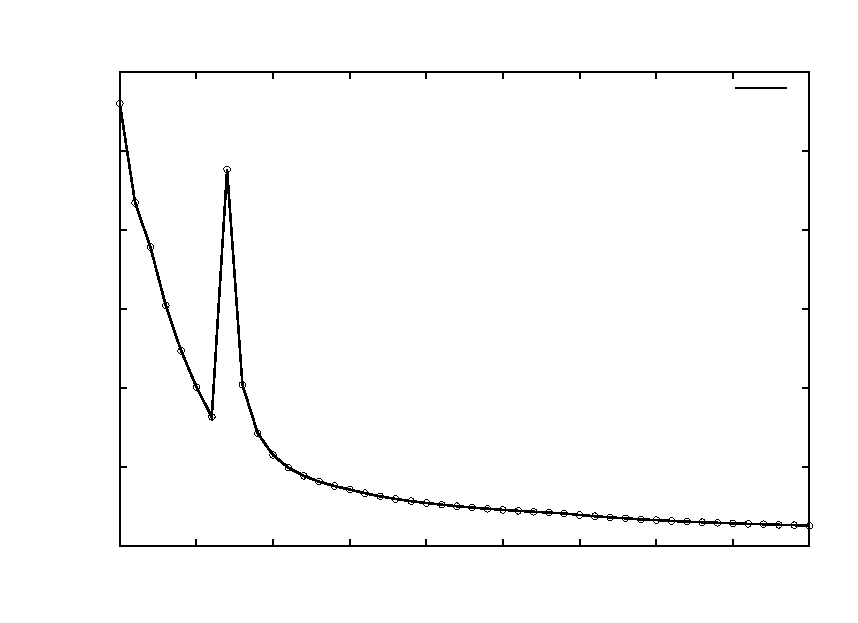
\includegraphics{./graph-02:convergence-grosso}}%
    \gplfronttext
  \end{picture}%
\endgroup

\end{Gráfico}

\begin{Gráfico}
	% GNUPLOT: LaTeX picture with Postscript
\begingroup
  \fontfamily{phv}%
  \selectfont
\definecolor{t}{rgb}{0.5,0.5,0.5}
  \makeatletter
  \providecommand\color[2][]{%
    \GenericError{(gnuplot) \space\space\space\@spaces}{%
      Package color not loaded in conjunction with
      terminal option `colourtext'%
    }{See the gnuplot documentation for explanation.%
    }{Either use 'blacktext' in gnuplot or load the package
      color.sty in LaTeX.}%
    \renewcommand\color[2][]{}%
  }%
  \providecommand\includegraphics[2][]{%
    \GenericError{(gnuplot) \space\space\space\@spaces}{%
      Package graphicx or graphics not loaded%
    }{See the gnuplot documentation for explanation.%
    }{The gnuplot epslatex terminal needs graphicx.sty or graphics.sty.}%
    \renewcommand\includegraphics[2][]{}%
  }%
  \providecommand\rotatebox[2]{#2}%
  \@ifundefined{ifGPcolor}{%
    \newif\ifGPcolor
    \GPcolortrue
  }{}%
  \@ifundefined{ifGPblacktext}{%
    \newif\ifGPblacktext
    \GPblacktextfalse
  }{}%
  % define a \g@addto@macro without @ in the name:
  \let\gplgaddtomacro\g@addto@macro
  % define empty templates for all commands taking text:
  \gdef\gplbacktext{}%
  \gdef\gplfronttext{}%
  \makeatother
  \ifGPblacktext
    % no textcolor at all
    \def\colorrgb#1{}%
    \def\colorgray#1{}%
  \else
    % gray or color?
    \ifGPcolor
      \def\colorrgb#1{\color[rgb]{#1}}%
      \def\colorgray#1{\color[gray]{#1}}%
      \expandafter\def\csname LTw\endcsname{\color{white}}%
      \expandafter\def\csname LTb\endcsname{\color{black}}%
      \expandafter\def\csname LTa\endcsname{\color{black}}%
      \expandafter\def\csname LT0\endcsname{\color[rgb]{1,0,0}}%
      \expandafter\def\csname LT1\endcsname{\color[rgb]{0,1,0}}%
      \expandafter\def\csname LT2\endcsname{\color[rgb]{0,0,1}}%
      \expandafter\def\csname LT3\endcsname{\color[rgb]{1,0,1}}%
      \expandafter\def\csname LT4\endcsname{\color[rgb]{0,1,1}}%
      \expandafter\def\csname LT5\endcsname{\color[rgb]{1,1,0}}%
      \expandafter\def\csname LT6\endcsname{\color[rgb]{0,0,0}}%
      \expandafter\def\csname LT7\endcsname{\color[rgb]{1,0.3,0}}%
      \expandafter\def\csname LT8\endcsname{\color[rgb]{0.5,0.5,0.5}}%
    \else
      % gray
      \def\colorrgb#1{\color{black}}%
      \def\colorgray#1{\color[gray]{#1}}%
      \expandafter\def\csname LTw\endcsname{\color{white}}%
      \expandafter\def\csname LTb\endcsname{\color{black}}%
      \expandafter\def\csname LTa\endcsname{\color{black}}%
      \expandafter\def\csname LT0\endcsname{\color{black}}%
      \expandafter\def\csname LT1\endcsname{\color{black}}%
      \expandafter\def\csname LT2\endcsname{\color{black}}%
      \expandafter\def\csname LT3\endcsname{\color{black}}%
      \expandafter\def\csname LT4\endcsname{\color{black}}%
      \expandafter\def\csname LT5\endcsname{\color{black}}%
      \expandafter\def\csname LT6\endcsname{\color{black}}%
      \expandafter\def\csname LT7\endcsname{\color{black}}%
      \expandafter\def\csname LT8\endcsname{\color{black}}%
    \fi
  \fi
  \setlength{\unitlength}{0.0500bp}%
  \begin{picture}(7936.00,5668.00)%
    \gplgaddtomacro\gplbacktext{%
      \csname LTb\endcsname%
      \put(882,576){\makebox(0,0)[r]{\strut{} 1550}}%
      \put(882,1031){\makebox(0,0)[r]{\strut{} 1600}}%
      \put(882,1486){\makebox(0,0)[r]{\strut{} 1650}}%
      \put(882,1941){\makebox(0,0)[r]{\strut{} 1700}}%
      \put(882,2396){\makebox(0,0)[r]{\strut{} 1750}}%
      \put(882,2852){\makebox(0,0)[r]{\strut{} 1800}}%
      \put(882,3307){\makebox(0,0)[r]{\strut{} 1850}}%
      \put(882,3762){\makebox(0,0)[r]{\strut{} 1900}}%
      \put(882,4217){\makebox(0,0)[r]{\strut{} 1950}}%
      \put(882,4672){\makebox(0,0)[r]{\strut{} 2000}}%
      \put(882,5127){\makebox(0,0)[r]{\strut{} 2050}}%
      \put(990,396){\makebox(0,0){\strut{} 0.98}}%
      \put(1818,396){\makebox(0,0){\strut{} 1}}%
      \put(2645,396){\makebox(0,0){\strut{} 1.02}}%
      \put(3473,396){\makebox(0,0){\strut{} 1.04}}%
      \put(4301,396){\makebox(0,0){\strut{} 1.06}}%
      \put(5128,396){\makebox(0,0){\strut{} 1.08}}%
      \put(5956,396){\makebox(0,0){\strut{} 1.1}}%
      \put(6783,396){\makebox(0,0){\strut{} 1.12}}%
      \put(7611,396){\makebox(0,0){\strut{} 1.14}}%
      \put(144,2851){\makebox(0,0){\strut{}n}}%
      \put(4300,126){\makebox(0,0){\strut{}w}}%
      \put(4300,5397){\makebox(0,0){\strut{}Número de iterações para $\varepsilon =0.1$}}%
    }%
    \gplgaddtomacro\gplfronttext{%
      \csname LTb\endcsname%
      \put(6792,4974){\makebox(0,0)[r]{\strut{}n = 100}}%
    }%
    \gplbacktext
    \put(0,0){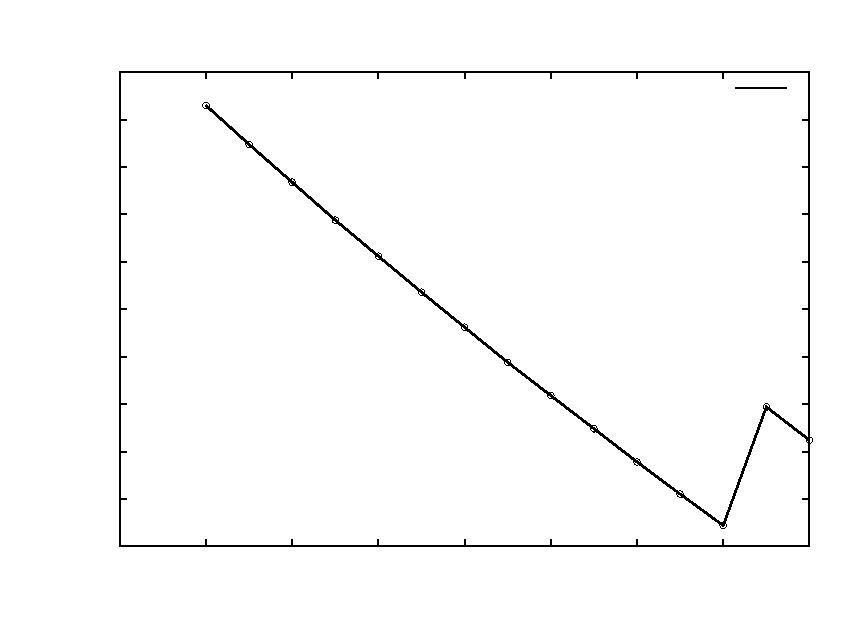
\includegraphics{./graph-03:convergence-fino}}%
    \gplfronttext
  \end{picture}%
\endgroup

\end{Gráfico}

\begin{Gráfico}
	% GNUPLOT: LaTeX picture with Postscript
\begingroup
  \fontfamily{phv}%
  \selectfont
\definecolor{t}{rgb}{0.5,0.5,0.5}
  \makeatletter
  \providecommand\color[2][]{%
    \GenericError{(gnuplot) \space\space\space\@spaces}{%
      Package color not loaded in conjunction with
      terminal option `colourtext'%
    }{See the gnuplot documentation for explanation.%
    }{Either use 'blacktext' in gnuplot or load the package
      color.sty in LaTeX.}%
    \renewcommand\color[2][]{}%
  }%
  \providecommand\includegraphics[2][]{%
    \GenericError{(gnuplot) \space\space\space\@spaces}{%
      Package graphicx or graphics not loaded%
    }{See the gnuplot documentation for explanation.%
    }{The gnuplot epslatex terminal needs graphicx.sty or graphics.sty.}%
    \renewcommand\includegraphics[2][]{}%
  }%
  \providecommand\rotatebox[2]{#2}%
  \@ifundefined{ifGPcolor}{%
    \newif\ifGPcolor
    \GPcolortrue
  }{}%
  \@ifundefined{ifGPblacktext}{%
    \newif\ifGPblacktext
    \GPblacktextfalse
  }{}%
  % define a \g@addto@macro without @ in the name:
  \let\gplgaddtomacro\g@addto@macro
  % define empty templates for all commands taking text:
  \gdef\gplbacktext{}%
  \gdef\gplfronttext{}%
  \makeatother
  \ifGPblacktext
    % no textcolor at all
    \def\colorrgb#1{}%
    \def\colorgray#1{}%
  \else
    % gray or color?
    \ifGPcolor
      \def\colorrgb#1{\color[rgb]{#1}}%
      \def\colorgray#1{\color[gray]{#1}}%
      \expandafter\def\csname LTw\endcsname{\color{white}}%
      \expandafter\def\csname LTb\endcsname{\color{black}}%
      \expandafter\def\csname LTa\endcsname{\color{black}}%
      \expandafter\def\csname LT0\endcsname{\color[rgb]{1,0,0}}%
      \expandafter\def\csname LT1\endcsname{\color[rgb]{0,1,0}}%
      \expandafter\def\csname LT2\endcsname{\color[rgb]{0,0,1}}%
      \expandafter\def\csname LT3\endcsname{\color[rgb]{1,0,1}}%
      \expandafter\def\csname LT4\endcsname{\color[rgb]{0,1,1}}%
      \expandafter\def\csname LT5\endcsname{\color[rgb]{1,1,0}}%
      \expandafter\def\csname LT6\endcsname{\color[rgb]{0,0,0}}%
      \expandafter\def\csname LT7\endcsname{\color[rgb]{1,0.3,0}}%
      \expandafter\def\csname LT8\endcsname{\color[rgb]{0.5,0.5,0.5}}%
    \else
      % gray
      \def\colorrgb#1{\color{black}}%
      \def\colorgray#1{\color[gray]{#1}}%
      \expandafter\def\csname LTw\endcsname{\color{white}}%
      \expandafter\def\csname LTb\endcsname{\color{black}}%
      \expandafter\def\csname LTa\endcsname{\color{black}}%
      \expandafter\def\csname LT0\endcsname{\color{black}}%
      \expandafter\def\csname LT1\endcsname{\color{black}}%
      \expandafter\def\csname LT2\endcsname{\color{black}}%
      \expandafter\def\csname LT3\endcsname{\color{black}}%
      \expandafter\def\csname LT4\endcsname{\color{black}}%
      \expandafter\def\csname LT5\endcsname{\color{black}}%
      \expandafter\def\csname LT6\endcsname{\color{black}}%
      \expandafter\def\csname LT7\endcsname{\color{black}}%
      \expandafter\def\csname LT8\endcsname{\color{black}}%
    \fi
  \fi
  \setlength{\unitlength}{0.0500bp}%
  \begin{picture}(7936.00,5668.00)%
    \gplgaddtomacro\gplbacktext{%
      \csname LTb\endcsname%
      \put(882,576){\makebox(0,0)[r]{\strut{} 5100}}%
      \put(882,1486){\makebox(0,0)[r]{\strut{} 5150}}%
      \put(882,2396){\makebox(0,0)[r]{\strut{} 5200}}%
      \put(882,3307){\makebox(0,0)[r]{\strut{} 5250}}%
      \put(882,4217){\makebox(0,0)[r]{\strut{} 5300}}%
      \put(882,5127){\makebox(0,0)[r]{\strut{} 5350}}%
      \put(990,396){\makebox(0,0){\strut{} 1.12}}%
      \put(1652,396){\makebox(0,0){\strut{} 1.122}}%
      \put(2314,396){\makebox(0,0){\strut{} 1.124}}%
      \put(2976,396){\makebox(0,0){\strut{} 1.126}}%
      \put(3638,396){\makebox(0,0){\strut{} 1.128}}%
      \put(4301,396){\makebox(0,0){\strut{} 1.13}}%
      \put(4963,396){\makebox(0,0){\strut{} 1.132}}%
      \put(5625,396){\makebox(0,0){\strut{} 1.134}}%
      \put(6287,396){\makebox(0,0){\strut{} 1.136}}%
      \put(6949,396){\makebox(0,0){\strut{} 1.138}}%
      \put(7611,396){\makebox(0,0){\strut{} 1.14}}%
      \put(144,2851){\makebox(0,0){\strut{}n}}%
      \put(4300,126){\makebox(0,0){\strut{}w}}%
      \put(4300,5397){\makebox(0,0){\strut{}Número de iterações para $\varepsilon =0.01$}}%
    }%
    \gplgaddtomacro\gplfronttext{%
      \csname LTb\endcsname%
      \put(6792,4974){\makebox(0,0)[r]{\strut{}n = 100}}%
    }%
    \gplbacktext
    \put(0,0){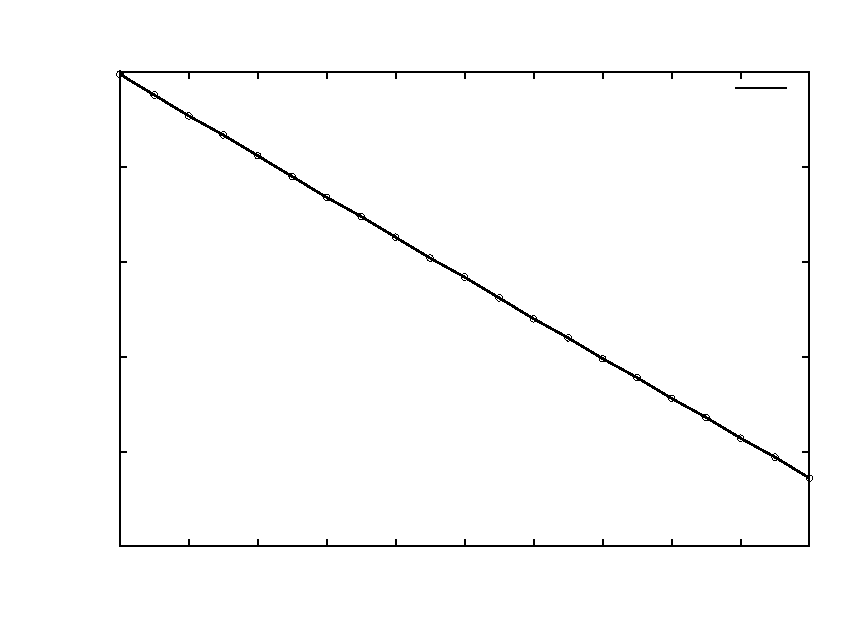
\includegraphics{./graph-04:convergence-fino-fino}}%
    \gplfronttext
  \end{picture}%
\endgroup

\end{Gráfico}

\begin{Gráfico}
	% GNUPLOT: LaTeX picture with Postscript
\begingroup
  \fontfamily{phv}%
  \selectfont
\definecolor{t}{rgb}{0.5,0.5,0.5}
  \makeatletter
  \providecommand\color[2][]{%
    \GenericError{(gnuplot) \space\space\space\@spaces}{%
      Package color not loaded in conjunction with
      terminal option `colourtext'%
    }{See the gnuplot documentation for explanation.%
    }{Either use 'blacktext' in gnuplot or load the package
      color.sty in LaTeX.}%
    \renewcommand\color[2][]{}%
  }%
  \providecommand\includegraphics[2][]{%
    \GenericError{(gnuplot) \space\space\space\@spaces}{%
      Package graphicx or graphics not loaded%
    }{See the gnuplot documentation for explanation.%
    }{The gnuplot epslatex terminal needs graphicx.sty or graphics.sty.}%
    \renewcommand\includegraphics[2][]{}%
  }%
  \providecommand\rotatebox[2]{#2}%
  \@ifundefined{ifGPcolor}{%
    \newif\ifGPcolor
    \GPcolortrue
  }{}%
  \@ifundefined{ifGPblacktext}{%
    \newif\ifGPblacktext
    \GPblacktextfalse
  }{}%
  % define a \g@addto@macro without @ in the name:
  \let\gplgaddtomacro\g@addto@macro
  % define empty templates for all commands taking text:
  \gdef\gplbacktext{}%
  \gdef\gplfronttext{}%
  \makeatother
  \ifGPblacktext
    % no textcolor at all
    \def\colorrgb#1{}%
    \def\colorgray#1{}%
  \else
    % gray or color?
    \ifGPcolor
      \def\colorrgb#1{\color[rgb]{#1}}%
      \def\colorgray#1{\color[gray]{#1}}%
      \expandafter\def\csname LTw\endcsname{\color{white}}%
      \expandafter\def\csname LTb\endcsname{\color{black}}%
      \expandafter\def\csname LTa\endcsname{\color{black}}%
      \expandafter\def\csname LT0\endcsname{\color[rgb]{1,0,0}}%
      \expandafter\def\csname LT1\endcsname{\color[rgb]{0,1,0}}%
      \expandafter\def\csname LT2\endcsname{\color[rgb]{0,0,1}}%
      \expandafter\def\csname LT3\endcsname{\color[rgb]{1,0,1}}%
      \expandafter\def\csname LT4\endcsname{\color[rgb]{0,1,1}}%
      \expandafter\def\csname LT5\endcsname{\color[rgb]{1,1,0}}%
      \expandafter\def\csname LT6\endcsname{\color[rgb]{0,0,0}}%
      \expandafter\def\csname LT7\endcsname{\color[rgb]{1,0.3,0}}%
      \expandafter\def\csname LT8\endcsname{\color[rgb]{0.5,0.5,0.5}}%
    \else
      % gray
      \def\colorrgb#1{\color{black}}%
      \def\colorgray#1{\color[gray]{#1}}%
      \expandafter\def\csname LTw\endcsname{\color{white}}%
      \expandafter\def\csname LTb\endcsname{\color{black}}%
      \expandafter\def\csname LTa\endcsname{\color{black}}%
      \expandafter\def\csname LT0\endcsname{\color{black}}%
      \expandafter\def\csname LT1\endcsname{\color{black}}%
      \expandafter\def\csname LT2\endcsname{\color{black}}%
      \expandafter\def\csname LT3\endcsname{\color{black}}%
      \expandafter\def\csname LT4\endcsname{\color{black}}%
      \expandafter\def\csname LT5\endcsname{\color{black}}%
      \expandafter\def\csname LT6\endcsname{\color{black}}%
      \expandafter\def\csname LT7\endcsname{\color{black}}%
      \expandafter\def\csname LT8\endcsname{\color{black}}%
    \fi
  \fi
  \setlength{\unitlength}{0.0500bp}%
  \begin{picture}(7936.00,5668.00)%
    \gplgaddtomacro\gplbacktext{%
      \csname LTb\endcsname%
      \put(990,576){\makebox(0,0)[r]{\strut{} 12040}}%
      \put(990,1082){\makebox(0,0)[r]{\strut{} 12060}}%
      \put(990,1587){\makebox(0,0)[r]{\strut{} 12080}}%
      \put(990,2093){\makebox(0,0)[r]{\strut{} 12100}}%
      \put(990,2599){\makebox(0,0)[r]{\strut{} 12120}}%
      \put(990,3104){\makebox(0,0)[r]{\strut{} 12140}}%
      \put(990,3610){\makebox(0,0)[r]{\strut{} 12160}}%
      \put(990,4116){\makebox(0,0)[r]{\strut{} 12180}}%
      \put(990,4621){\makebox(0,0)[r]{\strut{} 12200}}%
      \put(990,5127){\makebox(0,0)[r]{\strut{} 12220}}%
      \put(1098,396){\makebox(0,0){\strut{} 1.131}}%
      \put(2028,396){\makebox(0,0){\strut{} 1.132}}%
      \put(2959,396){\makebox(0,0){\strut{} 1.133}}%
      \put(3889,396){\makebox(0,0){\strut{} 1.134}}%
      \put(4820,396){\makebox(0,0){\strut{} 1.135}}%
      \put(5750,396){\makebox(0,0){\strut{} 1.136}}%
      \put(6681,396){\makebox(0,0){\strut{} 1.137}}%
      \put(7611,396){\makebox(0,0){\strut{} 1.138}}%
      \put(144,2851){\makebox(0,0){\strut{}n}}%
      \put(4354,126){\makebox(0,0){\strut{}w}}%
      \put(4354,5397){\makebox(0,0){\strut{}Número de iterações para $\varepsilon =0.001$}}%
    }%
    \gplgaddtomacro\gplfronttext{%
      \csname LTb\endcsname%
      \put(6792,4974){\makebox(0,0)[r]{\strut{}n = 100}}%
    }%
    \gplbacktext
    \put(0,0){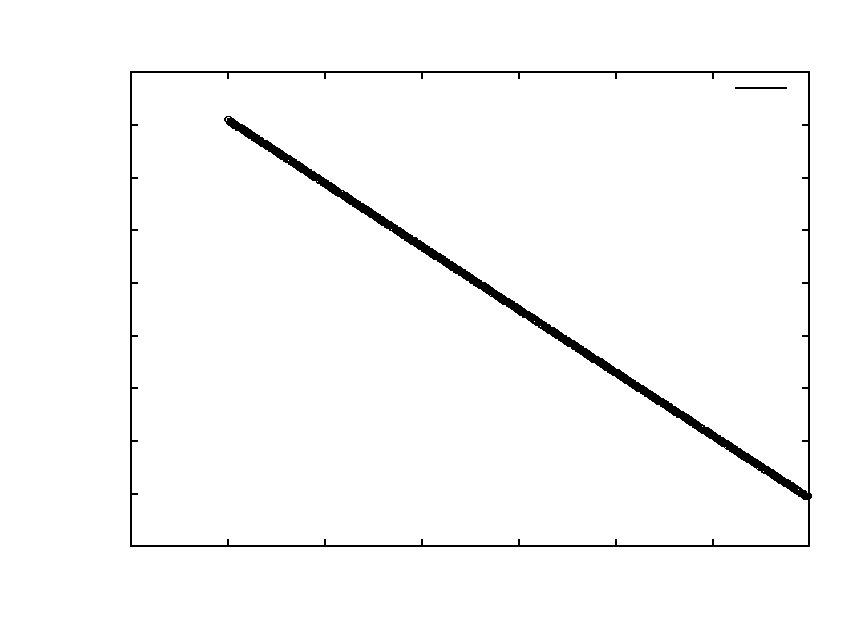
\includegraphics{./graph-05:convergence-fino-fino-fino}}%
    \gplfronttext
  \end{picture}%
\endgroup

\end{Gráfico}
%@@@@@@@@@@@@@@@@@@@@@@@@@@@@@@@@@@@@@@@@@@@@@@@@@@@@@@@@@@@
%@@@@@@@@@@@@@@       REFERÊNCIAS     @@@@@@@@@@@@@@@@@@@@@@
%@@@@@@@@@@@@@@@@@@@@@@@@@@@@@@@@@@@@@@@@@@@@@@@@@@@@@@@@@@@
\begin{thebibliography}{9}    
	 \bibitem{fis4-serway}
  		JEWETT, J.W.; SERWAY, R.A.
  		\emph{Física para cientistas e engenheiros} volume 4 : Luz, Óptica e Física Moderna.
 		 8ª ed.
 		 São Paulo : Cengage Learning, 2012.
 		 
 	 \bibitem{fis4-halliday}
  		HALLIDAY, D.; RESNICK, R. ; WALKER.
  		\emph{Fundamentos de Física} volume 4
 		 8ª ed.
 		 Rio de Janeiro : LTC, 2009.
 	
 	\bibitem{wiki:inverso_do_quadrado}
 			Wikipedia. Inverse-square law . Disponível em: http://en.wikipedia.org/wiki/Inverse-square$\_$law. Acesso em: 29 de maio de 2013

\end{thebibliography}



\end{document}
